% Adjust these for the path of the theme and its graphics, relative to this file
%\usepackage{beamerthemeFalmouthGamesAcademy}
\usepackage{../../beamerthemeFalmouthGamesAcademy}
\usepackage{multimedia}
\graphicspath{ {../../} }

% Default language for code listings
\lstset{language=C++,
	morekeywords={each,in,nullptr,int32, TCHAR, uint8, int8, uint16, int16,
		uint32, int32, uint64, int64, PTRINT, UObject. AActor, SWidget, FName,
		FString, UClass, USoundCue, UTexture}
}

% For strikethrough effect
\usepackage[normalem]{ulem}
\usepackage{wasysym}
\usepackage{listings}
\usepackage{pdfpages}
\usepackage[T1]{fontenc} 

% http://www.texample.net/tikz/examples/state-machine/
\usetikzlibrary{arrows,automata}

\newcommand{\modulecode}{GAM250}\newcommand{\moduletitle}{Advanced Games Programming }\newcommand{\sessionnumber}{2}

\begin{document}
	\title{\sessionnumber: Data Structures and Collections}
	\subtitle{\modulecode: \moduletitle}
	
	\frame{\titlepage}
	
	\begin{frame}
	\frametitle{Learning outcomes}
	\begin{itemize}
		\item \textbf{Understand} the various collection classes in C\#
		\item \textbf{Compare} the collection classes
		\item \textbf{Implement} an application which uses collection classes
	\end{itemize}
\end{frame}

\part{Common Data Structures}
\frame{\partpage}

\begin{frame}{Introduction}
	\begin{itemize}
		\pause \item In Programming we have concept of reusable data structures which can be used to build applications
		\pause \item These can be used in order to build larger systems (e.g. Inventory Systems, AI Navigation etc)
		\pause \item Most programming languages have these built in
		\pause \item Before writing any system you should always examine these data structures and pick the appropriate one for your Use Case 
	\end{itemize}
\end{frame}
\part{Big-O-Notation}
\frame{\partpage}

\begin{frame}{What is Big 'O' Notation}
\begin{itemize}
	\pause \item The efficiency of an algorithm can be gauged by how long it takes
	\pause \item This is know as \textbf{Time Complexity}
	\pause \item \textbf{Big O Notation} is used to describe this
\end{itemize}
\end{frame}

\begin{frame}{Constant - O(1)}
	\begin{center}
		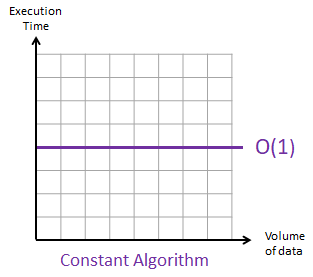
\includegraphics[height=0.8\textheight]{ConstantComplexity}
	\end{center}
\end{frame}

\begin{frame}{Linear - O(n)}
	\begin{center}
		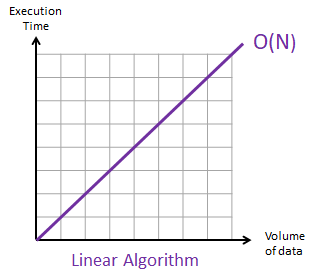
\includegraphics[height=0.8\textheight]{LinearComplexity}
	\end{center}
\end{frame}

\begin{frame}{Logarithmic - O(log(n))}
	\begin{center}
		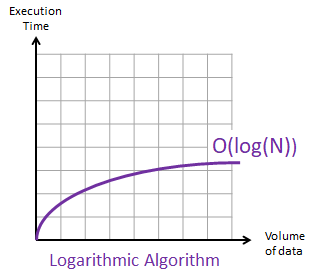
\includegraphics[height=0.8\textheight]{LogComplexity}
	\end{center}
\end{frame}

\begin{frame}{Big O Cheatsheet}
	\begin{center}
	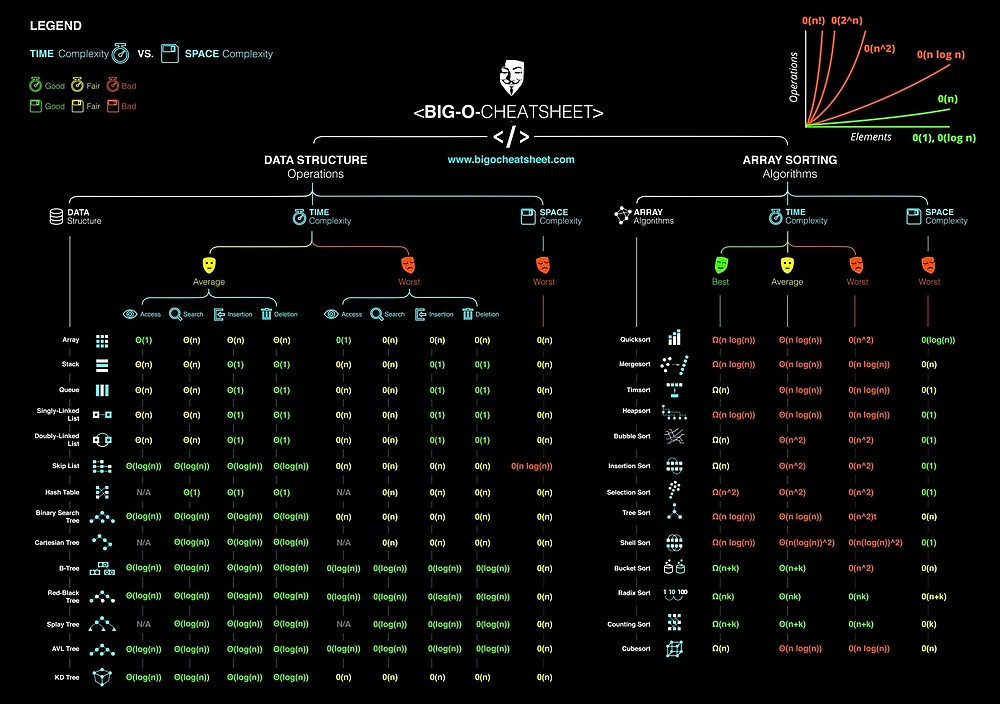
\includegraphics[height=0.8\textheight]{BigOCheatSheet}
	\end{center}
\end{frame}
\part{Dynamic Array}
\frame{\partpage}

\begin{frame}{The Problem}
	\begin{itemize}
		\pause \item Arrays in C\# are fixed in size
		\pause \item During development you need to know exactly how many item are going to be in the array
		\pause \item If you need to add elements and you don't have enough space, you will need to carry out the following
		\begin{itemize}
			\pause \item Create a new array of the appropriate size 
			\pause \item Copy elements from the old array into this new one
			\pause \item Destroy the old array
			\pause \item Add in the new element
		\end{itemize}
		\pause \item The above process can be quite costly
	\end{itemize}
\end{frame}

\begin{frame}{The Solution}
	\begin{itemize}
		\pause \item Luckily in most programming languages we have a Data Structure which grows in size when we require it 
		\begin{itemize}
			\pause \item In C\# we have the \textbf{List} class
		\end{itemize}
		\pause \item These classes have the same properties as an array
		\begin{itemize}
			\pause \item Items are located contiguously in memory 
			\pause \item We can randomly access elements using an index
			\pause \item We can iterate through each element
		\end{itemize}
		\pause \item You should consider using a Dynamic Array over a normal array
		\pause \item One caveat, Dynamic Arrays are slightly more expensive!
	\end{itemize}
\end{frame}

\begin{frame}{Use Case}
	\begin{itemize}
		\pause \item Manage Enemies as they are spawned into the scene
		\pause \item Keep track of players as they are added into the game
		\pause \item Inventory systems 
	\end{itemize}
\end{frame}

\begin{frame}[fragile]{C\# List
	 Example}
			\begin{lstlisting}
			List<int> scores=new List<int>();
			scores.Add(100);
			scores.Add(200);
			foreach(int score in scores)
			{
				Debug.Log("Score is "+score.ToString());
			}
			int player1Score=scores[0];
			scores.Remove(100);
			\end{lstlisting}
\end{frame}

\begin{frame}{Additional Notes}
	\begin{itemize}
		\pause \item Try to avoid insertion/deleting in the middle of the collection
		\pause \item Searching the collection is linear and will increase as more elements are added (O(n))
		\pause \item insertion/deleting at the end of the collection is constant in performance (O(1)) 
	\end{itemize}
\end{frame}

\part{Generic Types}
\frame{\partpage}

\begin{frame}{Quick Aside - Generic Programming}
	\begin{itemize}
		\pause \item Generic Programming is where you write one piece of code which operates on many different types
		\pause \item This uses a concept called Templates which act in proxy for the type
		\pause \item The Compiler then generates the code which uses the actual type
	\end{itemize}
\end{frame}

\begin{frame}{Look back at List}
	\begin{itemize}
		\pause \item In the previous section you would have noticed the following
		\begin{itemize}
			\pause \item List\textbf{\textless}int\textbf{\textgreater} 
		\end{itemize} 
		\pause \item These are know as generic parameters and you should insert the data type that the collection will handle (including your own data types aka classes and structs)
	\end{itemize}
\end{frame}

\begin{frame}{Generic Programming}
	\begin{itemize}
		\pause \item You can write your own generic classes and functions but this is beyond the scope of this class
		\pause \item C\# examples -
		\url{http://www.tutorialsteacher.com/csharp/csharp-generics}
		\pause \item Word of warning, it is often difficult to write generic code
		\pause \item If you have errors they are often difficult to isolate as the compiler messages are so cryptic
	\end{itemize}
\end{frame}
\part{Linked List}
\frame{\partpage}

\begin{frame}{The Problem}
	\begin{itemize}
		\pause \item You have started using a dynamic array and you have notice performance is poor on adding/removing
		 \pause \item You then realise that you are adding/removing elements from the middle of the collection
		 \pause \item You also realise that you don't require random access to elements in the collection
	\end{itemize}
\end{frame}

\begin{frame}{The Solution}
	\begin{itemize}
		\pause \item In this case a Linked List would be a better choice
		\begin{itemize}
			\pause \item In C\# we have the \textbf{LinkedList} class
		\end{itemize}
		\pause \item Linked Lists contain elements (called Nodes) which usually have a reference (or pointer) to the previous and next Node in the list
		\pause \item This means that there is a slight increase in memory needed when working with lists
	\end{itemize}
\end{frame}

\begin{frame}{Use Case}
	\begin{itemize}
		\pause \item If you AI character has to visit a series of waypoints, these could be stored in a list
		\pause \item Your Player has a number of quests they can try and complete
		\pause \item If the AI/Player carries an action and a number of systems need to be notified of the event 
	\end{itemize}
\end{frame}

\begin{frame}[fragile]{C\# Linked List
Example}
\begin{lstlisting}
	LinkedList<Transform> waypoints=new LinkedList<Transform>();
	
	waypoints.AddLast(GameObject.Find("Waypoint1").Transform);
	waypoints.AddLast(GameObject.Find("Waypoint2").Transform);
	waypoints.AddLast(GameObject.Find("Waypoint3").Transform);
	
	foreach(Transfrom t in waypoints)
	{
		Debug.Log("Waypoint Locations "+t.position.ToString());
	}
\end{lstlisting}
\end{frame}

\begin{frame}[fragile]{C\# Linked List
	Example}
\begin{lstlisting}
waypoints.AddFirst(GameObject.Find("Waypoint0").Transform);

LinkedListNode<Transform> waypoint2Node = linked.Find(GameObject.Find("Waypoint2"));
waypoints.AddAfter(waypoint2Node,GameObject.Find("SpecialQuest"));
\end{lstlisting}
\end{frame}


\begin{frame}{Additional Notes}
	\begin{itemize}
		\pause \item Linked Lists usually support constant time insertions and deletions in the collection (O(1))
		\pause \item Also perform better than dynamic arrays for moving elements around the collection
		\pause \item This feature means that Linked Lists are a good data structure if you need to sort your data
		\pause \item Main drawback of Linked Lists is that you can't have direct access to elements in the list, it takes linear time (O(n)) to access
	\end{itemize}
\end{frame}
\part{Queue}
\frame{\partpage}

\begin{frame}{The Problem}
	\begin{itemize}
		\pause \item If you need to visit items in a certain (e.g front to back)
		\pause \item Examples of this could be waypoints or commands to an AI character 
	\end{itemize}
\end{frame}

\begin{frame}{The Solution}
	\begin{itemize}
		\pause \item In this case a Queue would be a good choice
		\begin{itemize}
			\pause \item In C\# we have the \textbf{Queue} class
		\end{itemize}
		\pause \item This is \textbf{F}irst-\textbf{I}n-\textbf{L}ast-\textbf{O}ut data structure
		\pause \item You add elements to the end of the queue and you remove elements from the start
	\end{itemize}
\end{frame}

\begin{frame}{Use Case}
	\begin{itemize}
		\pause \item An RTS game where you can add orders to a unit, these are then carried out sequence
		\pause \item An RTS where you have a base which produces units
		\pause \item A spawning system, where you have to defeat enemies in a specific order
	\end{itemize}
\end{frame}

\begin{frame}[fragile]{C\# Queue
Example}
\begin{lstlisting}
Queue<GameObject> unitsToBuild=new Queue<GameObject>();

unitsToBuild.Enqeue(soliderPrefab);
unitsToBuild.Enqeue(builderPrefab);
unitsToBuild.Enqeue(tankPrefab);

foreach(GameObject go in unitsToBuild)
{
	Debug.Log("Units to build "+go.name);
}

\end{lstlisting}
\end{frame}


\begin{frame}[fragile]{C\# Queue
	Example}
\begin{lstlisting}
	GameObject nextUnitToBuild=unitsToBuild.Peek();
	
	unitsToBuild.Dequeue();
\end{lstlisting}
\end{frame}

\part{Stack}
\frame{\partpage}

\begin{frame}{The Problem}
	\begin{itemize}
		\pause \item If you need to manage the state of an AI character
		\pause \item If you need to implement a Undo system   
	\end{itemize}
\end{frame}

\begin{frame}{The Solution}
	\begin{itemize}
	\pause \item A Stack would be a good choice
	\begin{itemize}
		\pause \item In C\# we have the \textbf{Stack} class
	\end{itemize}
	\pause \item This is \textbf{L}ast-\textbf{I}n-\textbf{F}irst-\textbf{O}ut data structure
	\pause \item You add elements to the top of the stack and you remove elements from the top
\end{itemize}
\end{frame}

\begin{frame}[fragile]{C\# Stack
Example}
\begin{lstlisting}
Stack<Command> issuedCommands=new Stack<Command>();

issuedCommands.Push(new Command("Edit"));
issuedCommands.Push(new Command("Create"));
issuedCommands.Push(new Command("Update"));

\end{lstlisting}
\end{frame}

\begin{frame}[fragile]{C\# Stack
	Example}
\begin{lstlisting}
Command lastCommandIssued=issuedCommands.Peek();

Command lastCommandIssued=issuedCommands.Pop();
\end{lstlisting}
\end{frame}

\part{Associative Array: Dictionary}
\frame{\partpage}

\begin{frame}{The Problem}
	\begin{itemize}
		\pause \item If you need to store one unique copy of an element
		\pause \item You want to access an element via a key
		\pause \item You are doing lots of searches for an element
	\end{itemize}
\end{frame}

\begin{frame}{The Solution}
	\begin{itemize}
		\pause \item You should use an Associative array
		\begin{itemize}
			\pause \item In C\# we have the \textbf{Dictionary} class
		\end{itemize} 
		\pause \item These data structures are structured as key-value pair
		\pause \item It allows you to retrieve the items via the key
		\pause \item This makes it a good choice for looking up large data sets
	\end{itemize}
\end{frame}

\begin{frame}{Use Case}
	\begin{itemize}
		\pause \item If you are creating a resource management system for handling textures, models or other assets
		\pause \item Localisation system, each language is stored in an Associative Array
		\pause \item Unit Manager, a class to manage units created in the game
		\pause \item Save Game System
	\end{itemize}
\end{frame}

\begin{frame}[fragile]{C\# Dictionary
Example}
\begin{lstlisting}
Dictonary<string,int> highScoreTable=new Dictonary<string,int>();

highScores.Add("Brian",200);
highScores.Add("Sarah",2000);
highScores[Julia]=4000;

foreach(KeyValuePair<string,int> pair in highScoreTable)
{
	Debug.Log("High Score "+pair.Key+" "+pair.Value);
}
\end{lstlisting}
\end{frame}

\begin{frame}[fragile]{C\# Dictionary
	Example}
\begin{lstlisting}
if (highScores.ContainsKey("Brian"))
{
	int score=highScores["Brian"];
}

highScores.Remove("Sarah");
\end{lstlisting}
\end{frame}

\begin{frame}{Additional Notes}
\begin{itemize}
	\pause \item Iterating over a map has a slightly annoying syntax
	\pause \item Associative Arrays tend to have good performance for retrieval (O (log n))
	\pause \item If you add an item and its key already exists it may overwrite the value
\end{itemize}
\end{frame}
\part{Operations on collections}
\frame{\partpage}

\begin{frame}{Sorting}
	\begin{itemize}
		\pause \item Sorting is where we order the items in a collection in a specific order
		\pause \item There are a whole bunch of sorting algorithms including; Insertion sort, Heap sort, Quick sort (please read about these!)
		\pause \item In C\#, the best sorting algorithm will be picked depending on the size of the collection
		\pause \item In C++, this depends on the compiler implementation 
		\pause \item Most of the common data types don't need additional work
		\pause \item For custom classes, we have to write our own sorting algorithm
	\end{itemize}
\end{frame}

\begin{frame}{Sorting C\#}
	\begin{itemize}
		\pause \item There are few ways to sort a collection
		\begin{enumerate}
			\pause \item Provide a custom delegate function for the sort
			\pause \item Provide a custom class which inherits from \textbf{IComparer}
			\pause \item Your own class has to inherit from \textbf{IComparable}
		\end{enumerate}
		\pause \item Often you will use option 3 as the default sort
		\pause \item Which then be override by option 1 
	\end{itemize}
\end{frame}

\begin{frame}[fragile]{C\# Example - Sorting with Delegate }
\begin{lstlisting}
struct Character
{
	string name;
	int health;
	int strength;
}

//Adding omitted!
List<Character> characters=new List<Character>();

//Sort by health
characters.Sort(delegate (Character c1, Character c2)
{
	return (c1.health.CompareTo(c2.health));
});
\end{lstlisting}
\end{frame}

\begin{frame}[fragile]{C\# Example - Sorting with ICompareable }
\begin{lstlisting}
struct Character:IComparable<Character>
{
string name;
int health;
int strength;

// sort by name
 public int CompareTo(Character compareCharacter)
 {
 	return name.CompareTo(comareCharacter.name);
 }
}

//Adding omitted!
List<Character> characters=new List<Character>();

//Sort will use the CompareTo in the struct or class
characters.Sort()
\end{lstlisting}
\end{frame}

\begin{frame}{C\# - Points to note}
	\begin{itemize}
		\pause \item The \textbf{CompareTo} function returns an int which can be the following
		\begin{itemize}
			\pause \item Less than zero: The instance precedes the one passed in
			\pause \item Zero: The objects are in the same order
			\pause \item Greater than zero: The instance follows the one passed in
		\end{itemize} 
	\end{itemize}
\end{frame}

\part{Exercise}
\frame{\partpage}

\begin{frame}{Exercise 1 - Collections}
	\begin{enumerate}
		\item Download one of the following projects as a zip file
		\begin{itemize}
			\item BA Students - \url{https://github.com/Falmouth-Games-Academy/GAM160-Exercises}
			\item BSc Students - \url{https://github.com/Falmouth-Games-Academy/COMP140-Exercises}
		\end{itemize}
		\item Add additional items to the collection
		\item Display these to the screen
	\end{enumerate}
\end{frame}

\begin{frame}{Exercise 2 - Sorting}
\begin{enumerate}
	\item Write a default sort, so that the items are sorted by name
	\item Sort the collection when the \textbf{s} key is pressed
	\item Write another sort, to sort by score, trigger this off by a key press
	\item Write another sort, to sort by age, trigger this off by a key press
\end{enumerate}
\end{frame}

\begin{frame}{Exercise 3 - Searching}
\begin{enumerate}
	\item Investigate how to search for items in collections
	\item Add code to search for specific items in the collections 
	\item Add visual representation to show that the search has completed, this could be a colour change or just displaying the found item elsewhere on the screen
\end{enumerate}
\end{frame}

%\part{Singletongs}
\frame{\partpage}

\begin{frame}
\frametitle{References}
\url{https://unity3d.com/learn/tutorials/modules/intermediate/scripting/lists-and-dictionaries}
\url{https://www.101computing.net/big-o-notation/}
\url{http://bigocheatsheet.com/}
\end{frame}


\end{document}
